% !TEX root = MutationTestingSurvey.tex

\subsection{Automated Detection of Equivalent and Redundant Mutants}
\label{sec:dataequivalent}

Data-driven mutation operators may lead to the generation of both equivalent and redundant mutants.
In the data-driven context, \INDEX{equivalent mutants} consist of modified data (i.e., data altered by means of mutation operators) that do not lead to any noticeable difference in the output of the SUT with respect to the original version of the data.
Please note that an equivalent mutant differs in content from the original data (i.e., the data chunk has been altered).
The possible reasons why a mutant may not lead to noticeable differences in the output of the SUT are three. First, changes may go unnoticed because they alter portions of the data that is not read by the SUT. This includes cases in which mutations alter the structure of the input data in such a way that the resulting mutated data is different from the original but still respect the data format. This might happen, for example, when a mutation operator swaps the CDATA section of an XML file and the SUT ignores CDATA content. Second, mutations may alter some of the outputs of the SUT but the test suite oracles ignore that portion of the output. This might happen in a data acquisition system that copies the data payload of network packets in a database; in such a context, a data mutation that alters the message and update the packet checksum might go unnoticed because the SUT would simply copy the message content to the database and the test suite may simply check if the database contains a new message. Third, mutations may alter valid existing data but produce data that is still valid. This often reflect a poor choice of mutation operators; indeed, the selected mutation operators should guarantee to introduce a fault in the data exchanged by the system.




\INDEX{Redundant mutants} cause the same failures in the test suite. Two are the reasons for redundant mutants. First, the mutations alter different instances of a same data structure in the same way (e.g., delete a message in a sequence). Second, the mutations alter data chunks that are ignored by the oracles of the test suite.

\REVTWO{C35}{Concrete examples of equivalent and redundant mutants are provided in Figure~\ref{fig:data:quivalent}. In Figure~\ref{fig:data:quivalent}, \emph{Mutation 2} leads to an equivalent mutant since it 
generates a timestamp that is just one millisecond in the past, which is legal for the system under test. The value 2 for a timestamp, instead, leads to a failure because is considered too much in the past (see \emph{Mutation 1}). To address this problem, engineers should have configured the timestamp field to be mutated by a boundary condition operator (which generates values out of valid range) instead of a bit flipping operator. \emph{Mutation 3}  and \emph{Mutation 4}, instead, are redundant because they both generate a timestamp in the future (under the assumption that \emph{1584889773} captures the current time).}

\begin{figure}[h]
  \centering
    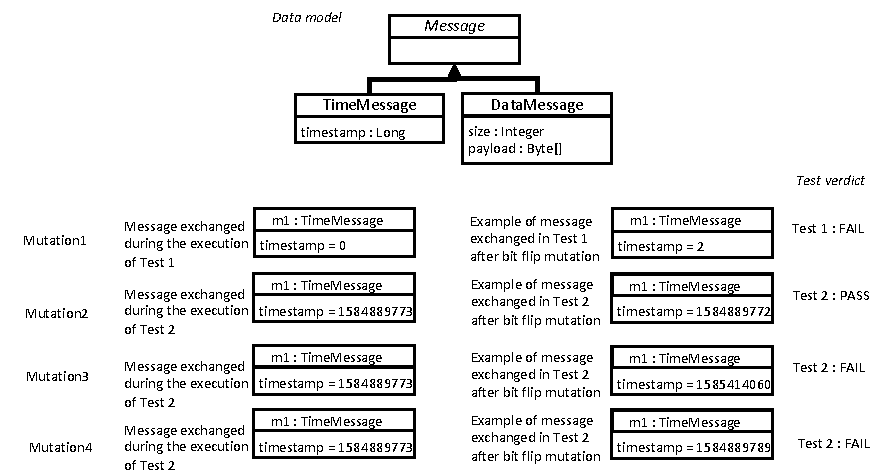
\includegraphics{images/DataDrivenEquivalent}
      \caption{Examples of data-driven mutations leading to equivalent and redundant mutants.}
      \label{fig:data:quivalent}
\end{figure}

Literature lacks approaches to directly target equivalent and redundant mutants. However, some of the solutions implemented in existing data mutation approaches might limit the presence of equivalent and redundant mutants. We observe three main solutions: (1) driving mutations by means of code-coverage, (2) driving mutations by means of coverage of model structure, and (3) use of model-based oracles.

Code-coverage-driven mutations are the ones implemented by many automated fuzzers such as 
MoWF~\cite{pham2016model} and AFL~\cite{gutmann2016fuzzing}.
MoWF aims to generate mutated data that triggers the execution of specific code locations. This is done by combining symbolic execution and meta-heuristic search.
Since each mutated input triggers a different code location, MoWF, in principle, should always lead to mutated inputs that make the software behave differently than with the original input or with other data mutants. However, it does not ensure that the changes in the internal behaviour of the software are reflected in one of its observable outputs.
Similarly to MoWF, AFL generates inputs that trigger different code locations. The main difference is that it does not target only specific code locations but it aims to exercise all the branches of the program. 
Similarly to MoWF, AFL does not guarantee that changes in the internal behaviour of the software are reflected in one of its observable outputs.
Similarly to AFL, any approach relying on meta-heuristic search that include coverage objectives in the fitness function (e.g.,~\cite{di2015evolutionary}) can limit the presence of equivalent and redundant mutants.


The coverage of the model structure enables the generation of mutations targeting different portions of a given data model.
For example, \emph{pFuzzer} generates valid inputs that cover diverse sets of lexical and syntactical features.
Other approaches~\cite{di2015generating} generate mutants that target different elements of the data structure.
By targeting different elements of the data, the generated mutants are unlikely to be redundant or equivalent. However, they do not ensure that such differences are reflected in the SUT observable outputs.


Model-based oracles, such as OCL constraints capturing expected outputs (e.g., error messages expected in the presence of a specific change of the data) enable the generation of mutants that are not equivalent and not redundant. For example, by ensuring that each mutant affects a model element referenced in a different OCL constraint and that the constraint is evaluated to true, model-based mutation approaches can guarantee that the data mutations lead to observable changes in the SUT output~\cite{di2015generating}.


